\chapter{Геометрия твердых тел}
\section{Геометрические примитивы}
Описание движения тела полностью абстрагировано от его формы
или, как принято выражаться, геометрии – это очень важно
уяснить для понимания внутренней архитектуры физического
движка.

Основными геометрическими примитивами используемыми в физических движках являются:
\begin{itemize}
 \item  луч 
 \item  плоскость,
 \item  полигон,
 \item  сфера,
 \item  треугольник,
 \end{itemize}
Для реализации более сложных геометрических тел используется композиция тел представленных выше.

Рассмотрим более подробно один основных из геометрических примитивов --- сферу.
Сфера может быть описана в пространстве положением своего геометрического цента(он же является и центром масс)
и радиуса. Таким образом для описания сферы достаточно 4 компонент : вектора положения центра сферы( 3 компоненты) и радиуса сферы.

%TODO Рассмотреть большее количество геометрически примитивов

\section{Обнаружение пересечений геометрических тел}
Реализации твердого тела и геометрического объекта как правило раздельны --- геометрия тела играет роль только в
процессе обнаружения столкновений, рассматриваемый ниже.

Модули обнаружения столкновений ($collision$ $detection$) и реагирования на столкновения ($collision$ $responce$) представляют 
собой ключевые компоненты любого физического движка. Именно они в процессе симуляции осуществляют главную нагрузку на
процессор, и именно от них требуется максимальная точность.

Методы обнаружения столкновений подразделяются на две категории: статические и динамические. В первом случае
движение тел рассматривается как последовательность «квантовых скачков» – проверка на пересечение двух геометрий
производится в промежутках между скачками, как если бы объекты в этом время не двигались (то есть, имели нулевые
скорости). Основным допущением этого метода является временная когерентность системы – предполагается, что тела
обладают небольшими скоростями, и их позиции не меняются слишком резко с течением времени. Иными словами,
статическое обнаружение столкновений плохо подходит для моделирования, например, пушки, стреляющей в бетонную
стену: за шаг времени ($\Delta{t}$) снаряд пройдет расстояние, значительно превышающее толщину стены, и, следовательно,
попросту пролетит сквозь нее --- статическая проверка это столкновение не обнаружит.

Динамическое обнаружение столкновений использует другой метод, при котором учитывается скорость тела – движок
предсказывает, какое положение в пространстве займет объект на следующем шаге времени, если будет двигаться с той же
скоростью. Фактически, делается проверка на пересечение отрезка, представляющего собой траекторию движения тела, с
препятствием – вычисляется точка, в которой тело столкнется с этим препятствием, и на основании этой информации движок
делает соответствующие корректировки. К сожалению, динамический метод довольно сложен (особенно для
нетривиальных геометрий) и, в целом, плохо адаптирован для динамики как таковой – он чаще используется в кинематике.
Поэтому далее будет рассматриваться статический метода – он, при всех его недостатках, хорошо себя оправдывает в
большинстве физических ситуаций.

В физическом движке функция проверки столкновения между двумя объектами должна давать на выходе следующую
информацию:
\begin{itemize}
  \item точка столкновения (точка контакта)
  \item нормаль к поверхности столкновения в этой точке (нормаль контакта)
  \item глубина взаимного проникновения объектов
\end{itemize}
\begin{center}
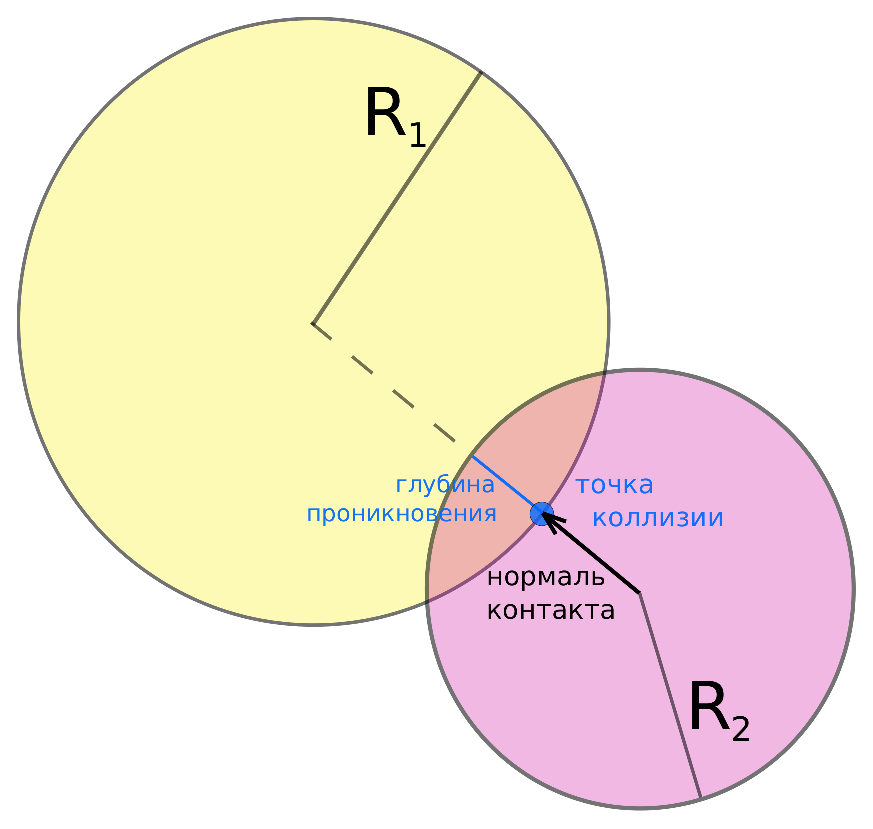
\includegraphics[scale=0.45]{./Collision/SphereCollision.eps}  \\
\textbf{Рис. Контакт двух сфер}
\end{center}
Эти три свойства, вкупе со ссылками на столкнувшиеся тела, дают новую сущность – контакт. Соответственно,
процесс обнаружения столкновений в терминологии физического движка также называют генерированием
контактов ($contact$ $generation$). В сложных движках на одно столкновение между двумя телами приходится несколько
контактов – так называемый $contact$ $manifold$. Далее будет рассматриваться простейший случай – столкновение сфер, где будет
достаточно одного контакта на пару столкнувшихся тел.
